%%%%%%%%%%%%%%%%%%%%%%%%%%%%%%%%%%%%%%%%%
% baposter Landscape Poster
% LaTeX Template
% Version 1.0 (11/06/13)
%
% baposter Class Created by:
% Brian Amberg (baposter@brian-amberg.de)
%
% This template has been downloaded from:
% http://www.LaTeXTemplates.com
%
% License:
% CC BY-NC-SA 3.0 (http://creativecommons.org/licenses/by-nc-sa/3.0/)
%
%%%%%%%%%%%%%%%%%%%%%%%%%%%%%%%%%%%%%%%%%

%----------------------------------------------------------------------------------------
%	PACKAGES AND OTHER DOCUMENT CONFIGURATIONS
%----------------------------------------------------------------------------------------

\documentclass[landscape,a0paper,fontscale=0.285]{baposter} % Adjust the font scale/size here
% Initial size : 0.285
\usepackage{graphicx} % Required for including images
\graphicspath{{figures/}} % Directory in which figures are stored

\usepackage{pgf}

\usepackage{amsmath} % For typesetting math
\usepackage{amssymb} % Adds new symbols to be used in math mode
\usepackage{mathrsfs}
%\usepackage{mathtools}

\usepackage{caption} 




\usepackage{url}

\usepackage{booktabs} % Top and bottom rules for tables
\usepackage{enumitem} % Used to reduce itemize/enumerate spacing
\usepackage{palatino} % Use the Palatino font
\usepackage[font=small,labelfont=bf]{caption} % Required for specifying captions to tables and figures

\usepackage{multicol} % Required for multiple columns
\setlength{\columnsep}{1.25em} % Slightly increase the space between columns
\setlength{\columnseprule}{0mm} % No horizontal rule between columns

\usepackage{tikz} % Required for flow chart
\usetikzlibrary{shapes,arrows} % Tikz libraries required for the flow chart in the template

\newcommand{\compresslist}{ % Define a command to reduce spacing within itemize/enumerate environments, this is used right after \begin{itemize} or \begin{enumerate}
\setlength{\itemsep}{1pt}
\setlength{\parskip}{0pt}
\setlength{\parsep}{0pt}
}




\definecolor{lightblue}{RGB}{66,66,111} % Defines the color used for content box headers

% Couleurs
\definecolor{marron}{rgb}{0.21,0.05,0.05} 
\definecolor{ivoire}{rgb}{1,0.97,0.90}
%\setbeamercolor{hauthb}{fg=white,bg=marron}
%\setbeamercolor{bashb}{fg=black,bg=ivoire}
\definecolor{gold}{rgb}{0.86,0.84,0.}
%\setbeamercolor{hautmb}{fg=black,bg=gold}
\definecolor{bleutitre}{rgb}{0,0,1}
\definecolor{vertbout}{rgb}{0.03,0.42,0.03}
%\setbeamercolor{hautbout}{fg=white,bg=vertbout}
\definecolor{vertsauge}{rgb}{0.41,0.82,0.54}
%\setbeamercolor{bassauge}{fg=black,bg=vertsauge}
\definecolor{bleupastel}{rgb}{0.34,0.45,0.6}
%\setbeamercolor{hautbp}{fg=white,bg=bleupastel}
\definecolor{lavande}{rgb}{0.59,0.51,0.93}
%\setbeamercolor{baslav}{fg=black,bg=lavande}
\definecolor{byzan}{rgb}{0.44,0.16,0.39}
%\setbeamercolor{hautbyz}{fg=white,bg=byzan}
\definecolor{dragee}{rgb}{0.99,0.75,0.82}
%\setbeamercolor{basdra}{fg=black,bg=dragee}
\definecolor{grisfonce}{rgb}{0.2,0.2,0.2}
%\setbeamercolor{hautgris}{fg=white,bg=grisfonce}
\definecolor{grispale}{rgb}{0.98,0.98,1}
%\setbeamercolor{basgris}{fg=black,bg=grispale}
\definecolor{redgeb}{RGB}{238,64,0}
%\setbeamercolor{hautgeb}{fg=white,bg=redgeb}
\definecolor{rougepale}{rgb}{1,0.4,0.4}
%\definecolor{bleufond}{rgb}{0.92,0.91,0.95}

%%%%%%%%%%%%%%%%%%%%%%%%%%%%%%%%%%%%%%%
% General color definitions
\definecolor{monrouge}{RGB}{199,21,11}
\definecolor{jaunemadison}{RGB}{239,155,15}
\definecolor{vertmadison}{RGB}{20,148,20}
\definecolor{kakimadison}{RGB}{121,137,51}
\definecolor{bleumadison}{RGB}{4,139,154}
\definecolor{rougemadison}{RGB}{157,38,29}
\definecolor{mauvemadison}{RGB}{172,30,68}
\definecolor{saumonmadison}{RGB}{248,142,85}
\definecolor{orangemadison}{RGB}{237,127,16}
\definecolor{rosemadison}{RGB}{249,66,158}
\definecolor{cerulmadison}{RGB}{15,157,232}
\definecolor{grismadison}{RGB}{206,206,206}
\definecolor{fauvemadison}{RGB}{173,79,9}

% Colors used for the theme
\definecolor{slidecol}{RGB}{157,38,29}
\definecolor{alertcol}{RGB}{71,12,117}
\definecolor{examplecol}{RGB}{0,51,105}

% Commands for colored texts
\newcommand{\vertcolb}[1]{\textcolor{vertmadison}{\textbf{#1}}}
\newcommand{\bleucolb}[1]{\textcolor{bleumadison}{\textbf{#1}}}
\newcommand{\rougecolb}[1]{\textcolor{rougemadison}{\textbf{#1}}}
\newcommand{\jaunecolb}[1]{\textcolor{jaunemadison}{\textbf{#1}}}
\newcommand{\bleucolm}[1]{\textcolor{bleumadison}{\mathbf{#1}}}
\newcommand{\vertcol}{\textcolor{vertmadison}}
\newcommand{\rougecol}{\textcolor{rougemadison}}
\newcommand{\bleucol}{\textcolor{bleumadison}}
\newcommand{\jaunecol}{\textcolor{jaunemadison}}
\newcommand{\examplec}{\textcolor{examplecol}}
\newcommand{\slidec}{\textcolor{slidecol}}
\newcommand{\alertc}{\textcolor{alertcol}}
\newcommand{\redcol}{\textcolor{monrouge}}
\newcommand{\examplecb}[1]{\textbf{\examplec{#1}}}
\newcommand{\slidecb}[1]{\textbf{\slidec{#1}}}
\newcommand{\alertb}[1]{\textbf{\alertc{#1}}}

\begin{document}

\begin{poster}
{
headerborder=closed, % Adds a border around the header of content boxes
colspacing=1em, % Column spacing
bgColorOne=white, % Background color for the gradient on the left side of the poster
bgColorTwo=white, % Background color for the gradient on the right side of the poster
borderColor=black, % Border color
headerColorTwo=white, % Background color for the header in the content boxes (left side)
headerColorOne=white, % Background color for the header in the content boxes (right side)
headerFontColor=black, % Text color for the header text in the content boxes
boxColorOne=white, % Background color of the content boxes
textborder=rectangle, % Format of the border around content boxes, can be: none, bars, coils, triangles, rectangle, rounded, roundedsmall, roundedright or faded
eyecatcher=true, % Set to false for ignoring the left logo in the title and move the title left
headerheight=0.2\textheight, % Height of the header
headershape=smallrounded, % Specify the rounded corner in the content box headers, can be: rectangle, small-rounded, roundedright, roundedleft or rounded
headerfont=\Large\bf\textsc, % Large, bold and sans serif font in the headers of content boxes
%textfont={\setlength{\parindent}{1.5em}}, % Uncomment for paragraph indentation
linewidth=1pt % Width of the border lines around content boxes
}
%----------------------------------------------------------------------------------------
%	TITLE SECTION 
%----------------------------------------------------------------------------------------
%
{
  \begin{minipage}{0.2\textwidth}
    
\includegraphics[height=2.5em]{dauphine}\\
    
\includegraphics[height=4.5em]{logomiles_white}\\[1ex]
    
\includegraphics[height=2.7em]{espci}%        
  \end{minipage}
}
% First university/lab logo on the left
{{\color{bleutitre}Experimental study of Neural ODE training with\\[0.5ex] adaptive solver
  for dynamical systems modeling}\vspace{1ex}} % Poster title
{  Alexandre Allauzen $^{1,2}$, Thiago Petrilli Maffei Dardis$^{2}$, Hannah Plath$^{2}$\\
  $^{1}$LAMSADE CNRS, Dauphine University-PSL, $^{2}$ESPCI-PSL
} % Author names
{} % Third logo



%----------------------------------------------------------------------------------------
%	REFERENCES
%----------------------------------------------------------------------------------------

% \headerbox{References}{name=references,column=0,span=4,above=bottom}{

% \renewcommand{\section}[2]{\vskip 0.05em} % Get rid of the default "References" section title
% %\nocite{*} % Insert publications even if they are not cited in the poster
% \small{ % Reduce the font size in this block
% \bibliographystyle{plain}
% \bibliography{refposter} % Use refposter.bib as the bibliography file
% }

% \small{\hfill\textit{\textbf{Funding for this research was provided by Subcontract 3F-30222 from Argonne National Laboratory and by a doctoral grant from Universit\'e Toulouse III Paul Sabatier.}}}

%}

\headerbox{Take-home message}{headerFontColor=red,name=abstract,span=2,column=0,row=0}{
aaa
}
\headerbox{Neural ODE and Fehlberg's method}{headerFontColor=bleutitre,name=eq,span=2,column=2,row=0}{
aaa
}
\headerbox{First round}{headerFontColor=bleutitre,name=exp1,span=2,column=0,row=0.4}{
  \vspace{-2ex}
  \begin{center}
    \hspace{-10ex}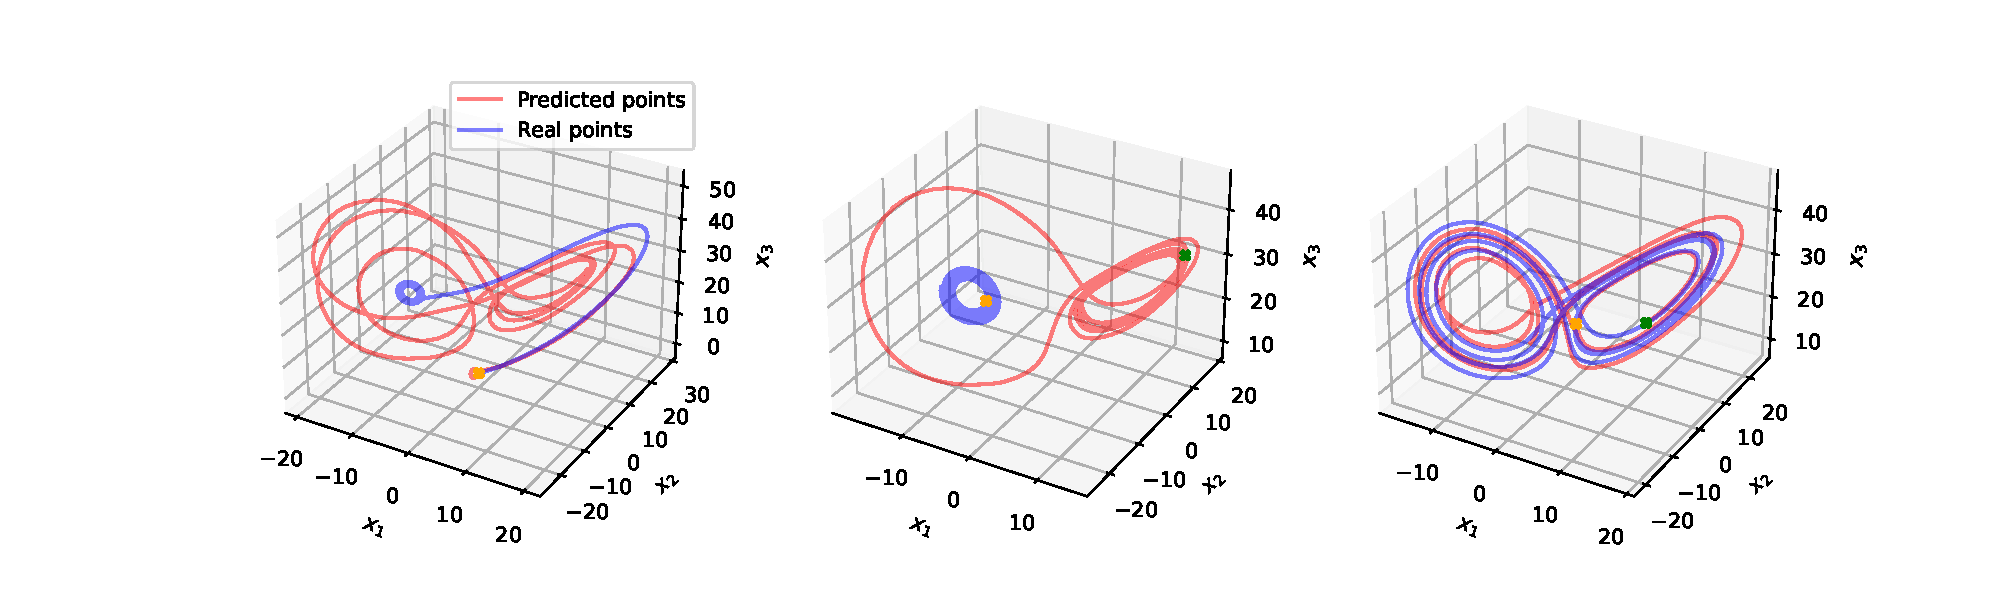
\includegraphics[width=0.8\textwidth]{../figs/baseline_lorenz_3}
    \\
    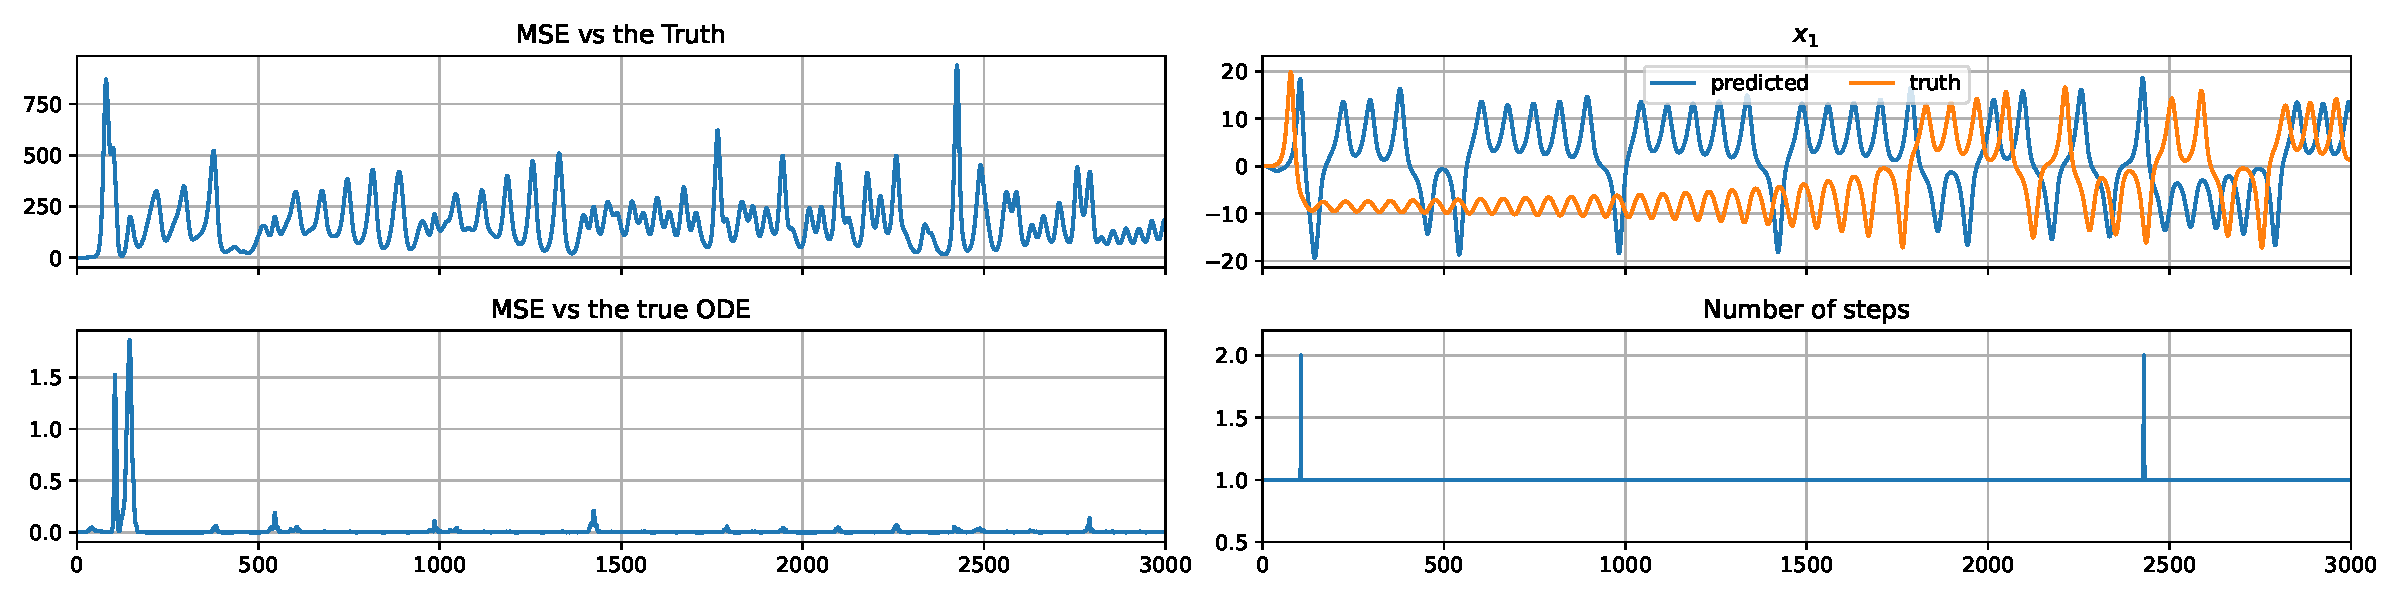
\includegraphics[width=0.8\textwidth]{../figs/baseline_time_series_2x2}
    \captionof{figure}{Time evolution of (from left to right and top to bottom):
    the MSE, the evolution of $x_1$, the MSE \textit{w.r.t} the true ODE of
    Lorenz'63, and  the number of
    steps.}
  \end{center}
}
\headerbox{Fehlberg's training}{headerFontColor=bleutitre,name=exp2,span=2,column=2,row=0.4}{
  \begin{minipage}{1.05\textwidth}
    \begin{center}
      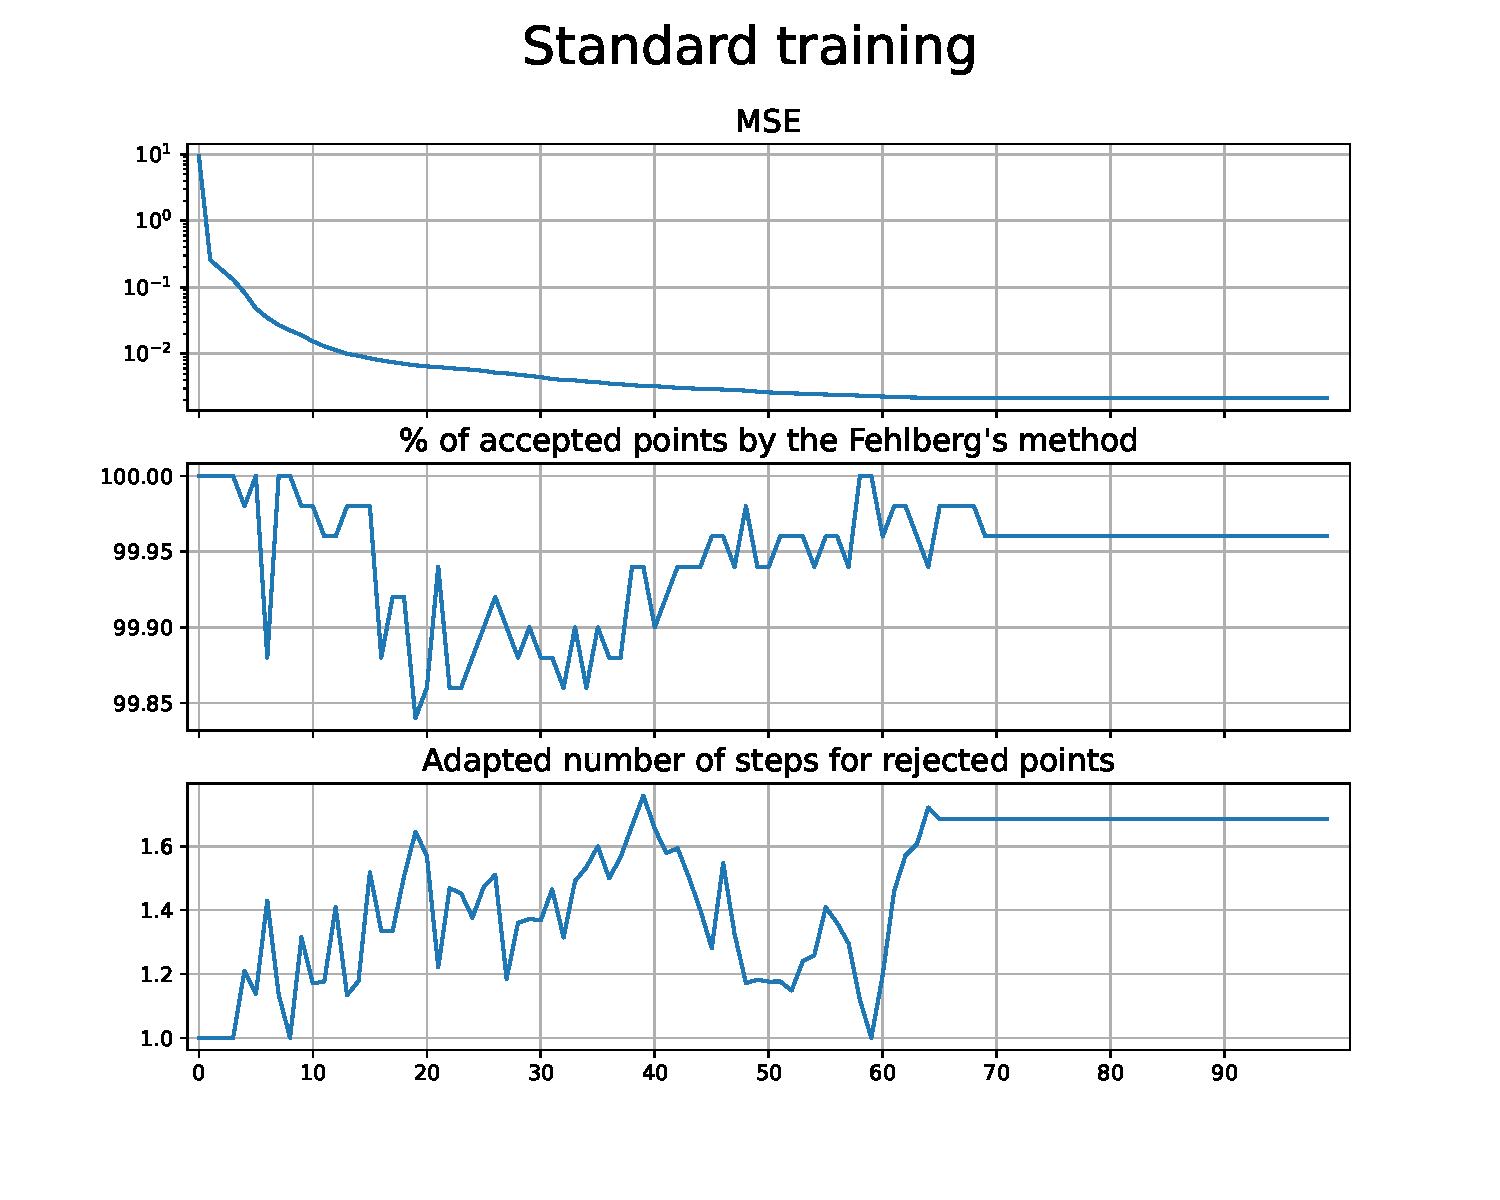
\includegraphics[width=0.49\textwidth]{../figs/batch_training}
      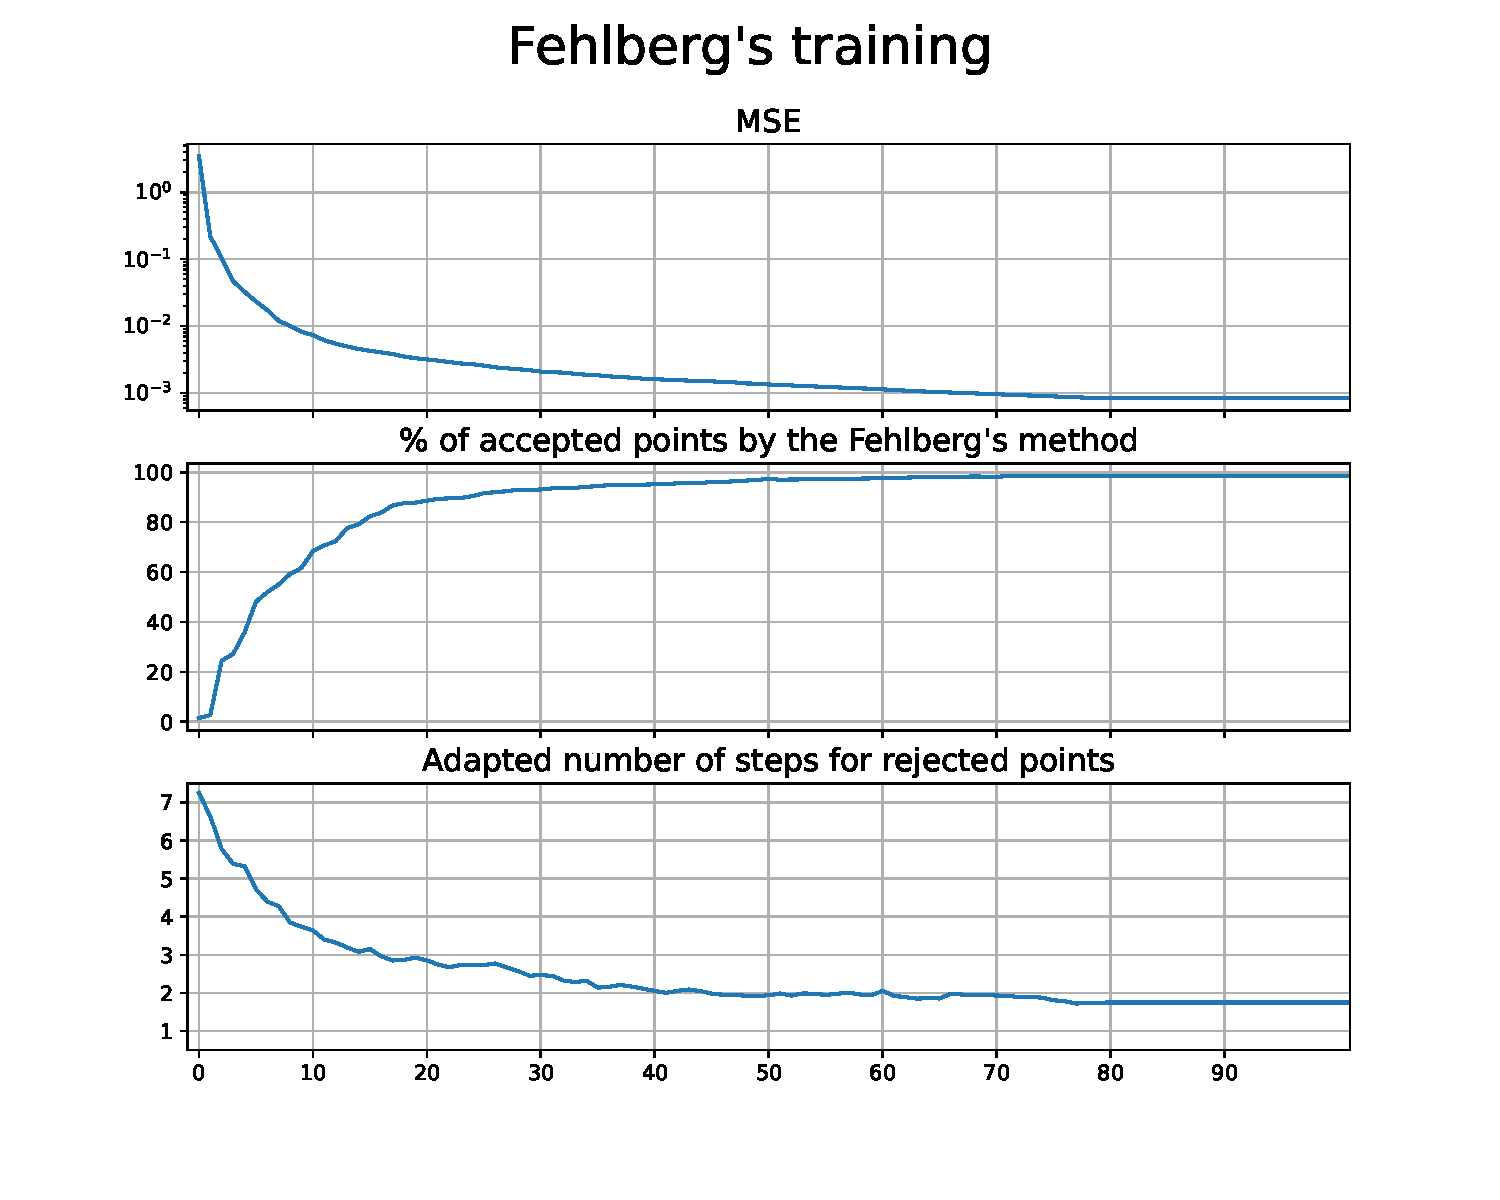
\includegraphics[width=0.49\textwidth]{../figs/fehlberg_training}
    \end{center}
  \end{minipage}
  \captionof{figure}{Time evolution for two training conditions of: the MSE loss; the percentage of
    accepted hypotheses $A_2$; the new number of steps for the rejected
    hypotheses (before rounding).}

}

\end{poster}
\end{document}